\clearpage
\subsection{Hardware}

\subsubsection{Mechanics}

\begin{figure}[ht]
    \begin{center}
        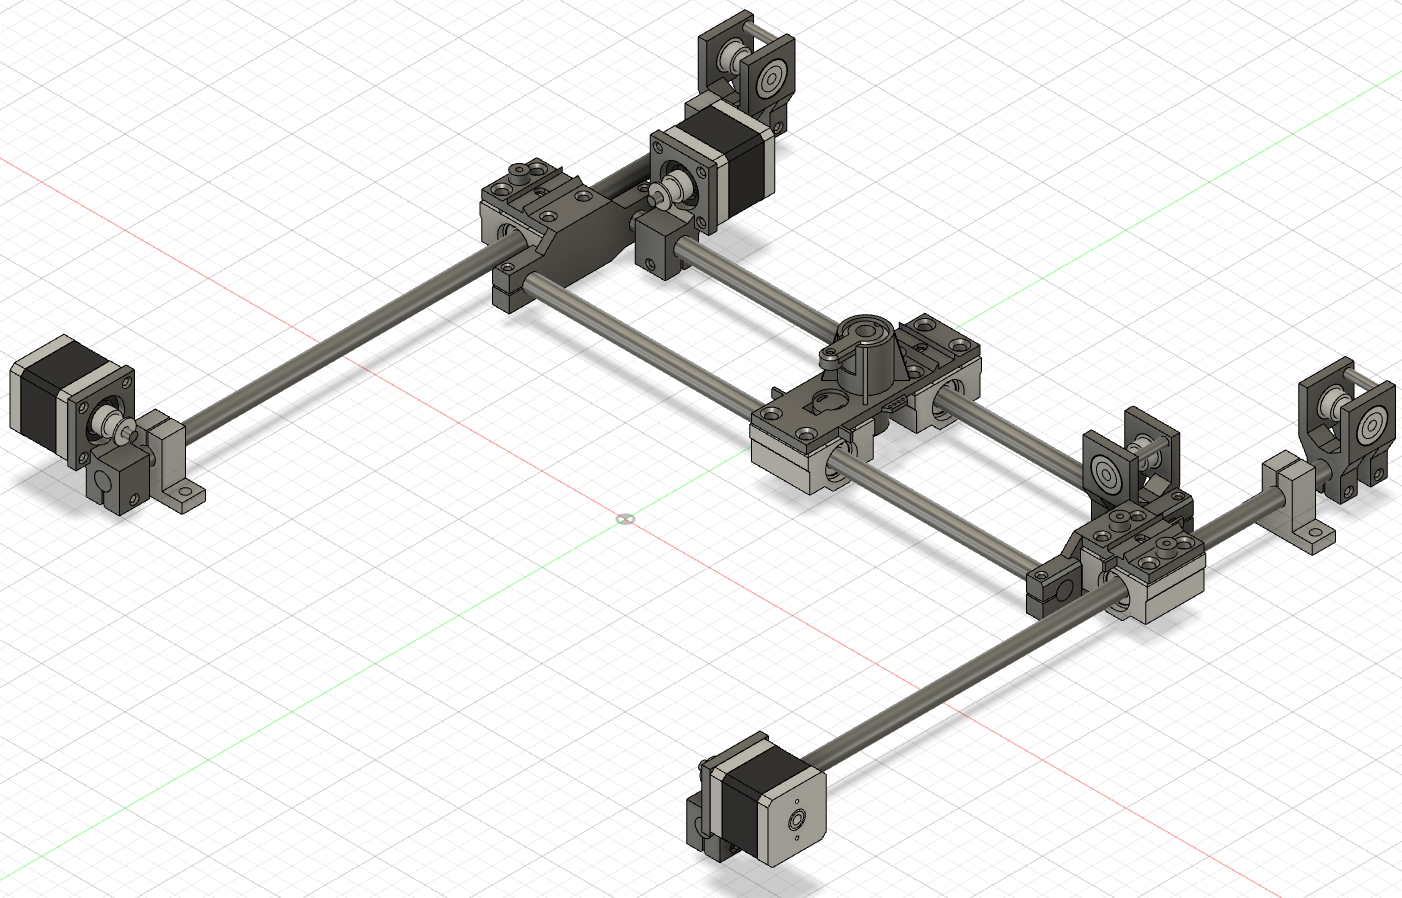
\includegraphics[width=\linewidth]{mechanics_overview}
        \caption{3D model of the mechanics}
    \end{center}
\end{figure}

The CNC machine consists of a set of moving platforms and cylindrical rails
mounted atop an 8-millimeter sheet of acrylic. It contains custom 3D-printed
parts used to join prefabricated metal components. The parts were designed in
Fusion 360 and printed with an Anycubic Photon S printer using the SLA 3D
printing technology.

Bolted directly to the base are two parallel rails, set 350 mm apart, which
guide movement in the Y axis. On each of the rails, mounted on top of a linear
bearing, is a platform which provides a mounting point for another pair of
rails. This pair, set 54 mm apart, guides movement in the X axis.

Placed across the second pair of rails, also mounted on linear bearings, is the
head assembly. It houses the interchangeable head, which holds the drawing
instrument, and guides its movement in the Z axis. It also provides a mounting
point for a small stepper motor coupled with the head.

Movement in the XY plane is driven by three stepper motors, coupled with their
respective platforms by timing belts. This enables movement at large speeds
while providing a reasonable amount of precision. Movement in the Z axis is
achieved with a leadscrew-type mechanism, where a small stepper motor with a
threaded shaft moves the head up and down.

\begin{figure}[ht]
    \centering
    \begin{minipage}{0.5\textwidth}
        \centering
        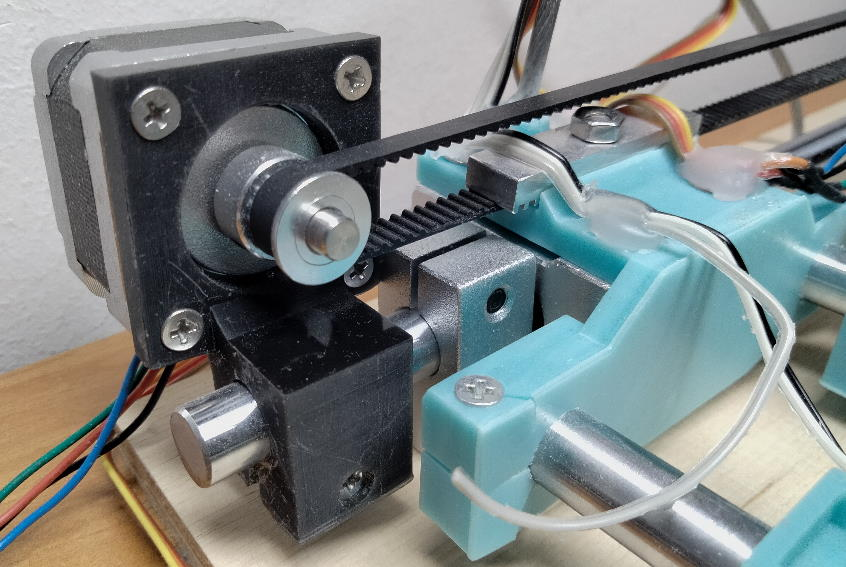
\includegraphics[width=0.9\textwidth]{xy_drive}
        \caption{XY drive using a timing belt}
    \end{minipage}\hfill
    \begin{minipage}{0.5\textwidth}
        \centering
        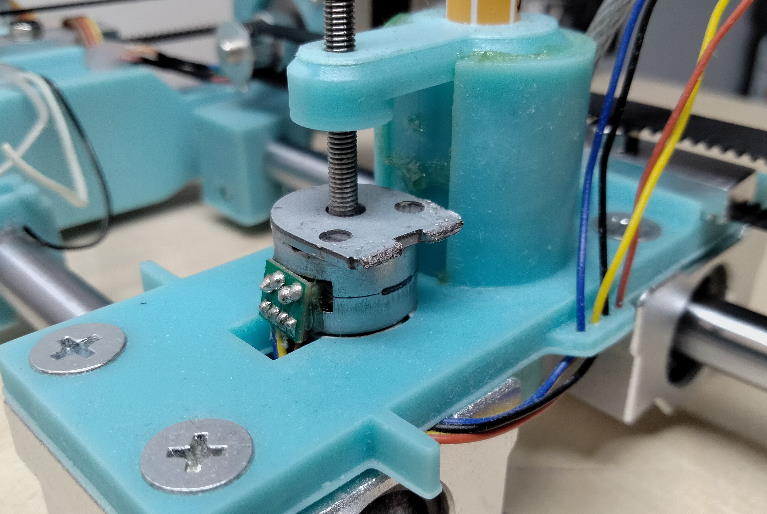
\includegraphics[width=0.9\textwidth]{z_drive}
        \caption{Z drive using a leadscrew}
    \end{minipage}
\end{figure}

The stepper motor used for XY movement is a JK35HY28-0504, a bipolar stepper
motor commonly used for CNC applications. It consumes 0.5 A per coil and
provides a torque of 0.1 Nm \cite{jk35hy28}. The smaller stepper motor used for
Z-axis movement is a generic no-brand bipolar motor available from online
retailers. It has been measured to provide sufficient torque at 0.2 A per coil.

The mechanical system described above is sufficient to achieve a full range of
motion in all three axes. Four stepper motors with a maximum current consumption
of 3.4 A may be controlled to achieve any toolpath. A microcontroller system,
shown in figure~\ref{schematic}, was designed to perform this task. The
circuit schematic and its corresponding PCB were created in KiCad.

\clearpage
\begin{sidewaysfigure}[ht]
    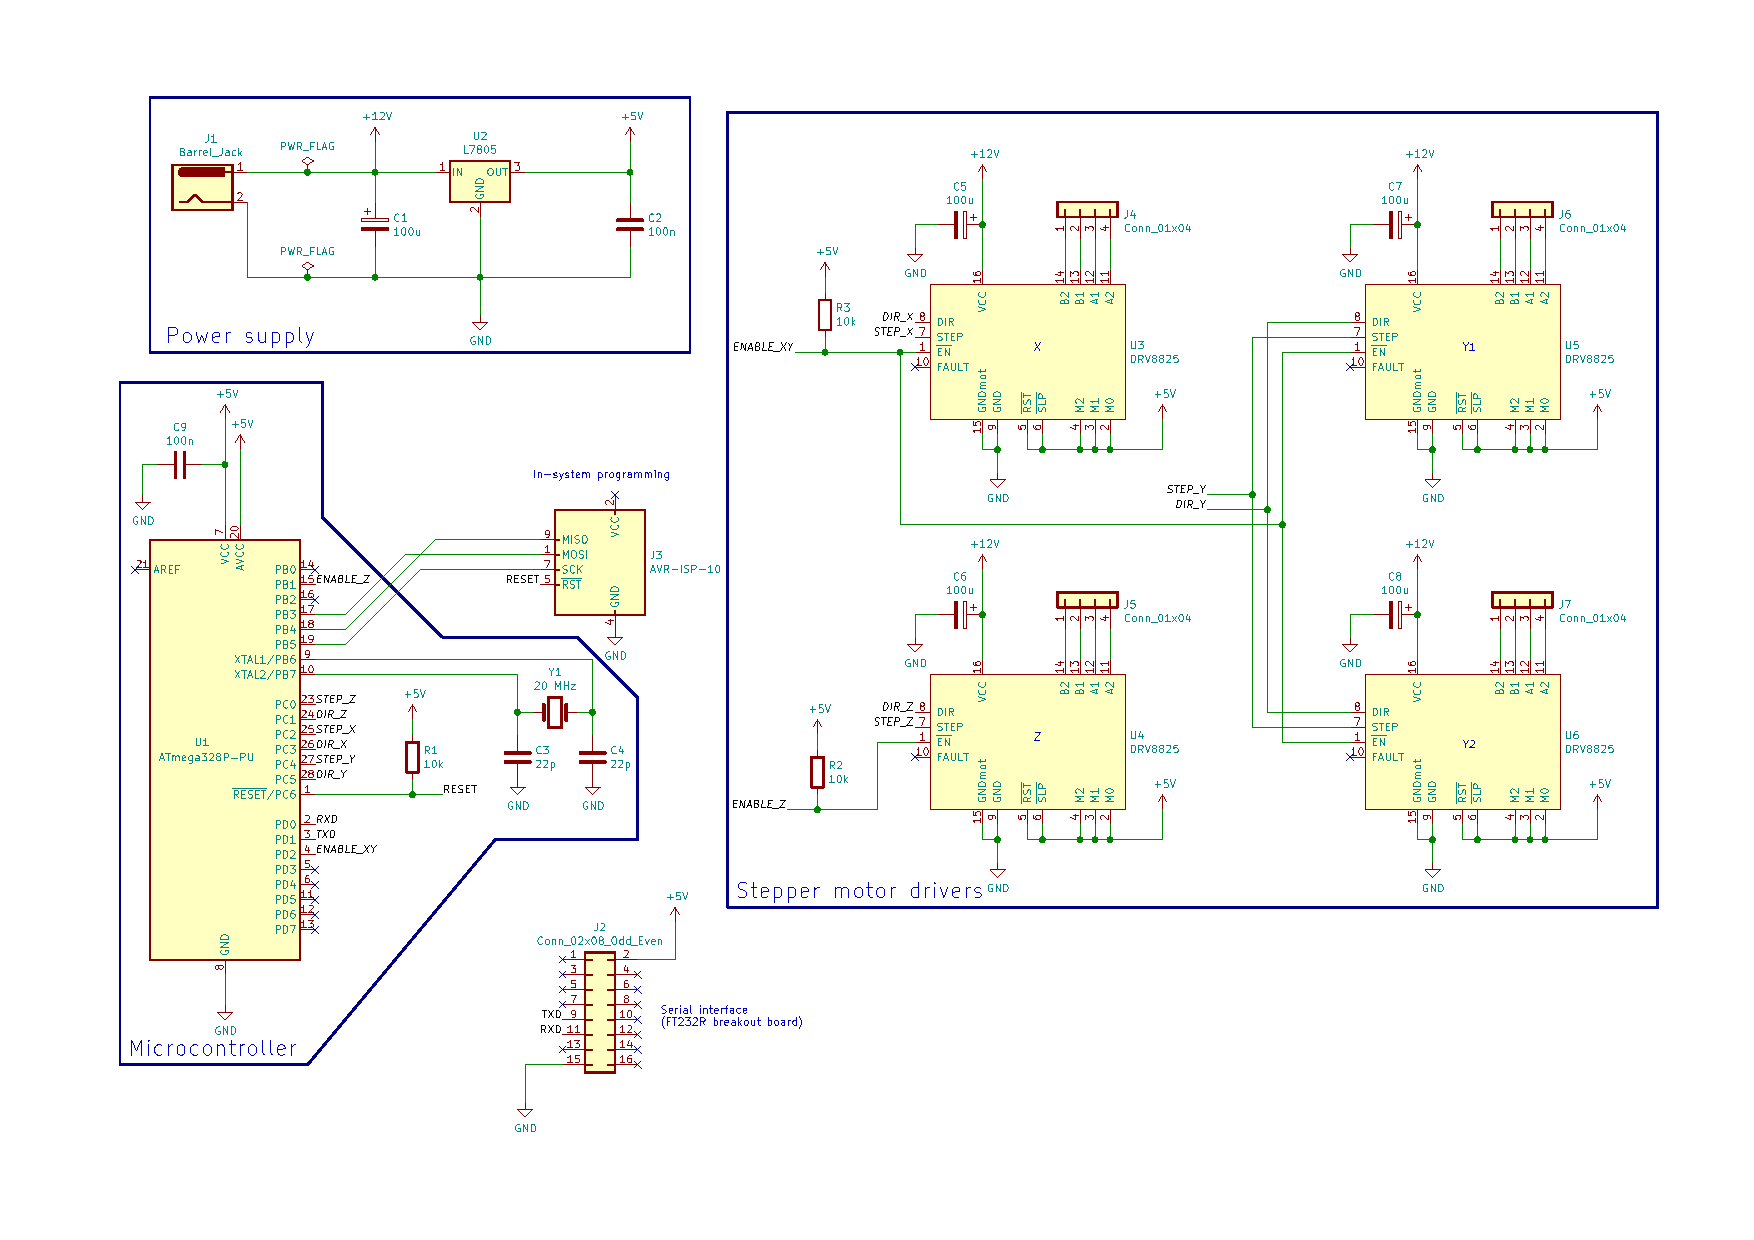
\includegraphics[width=\linewidth]{schematic}
    \caption{Schematic of the microcontroller system}
    \label{schematic}
\end{sidewaysfigure}

\clearpage

\subsubsection{Motor drivers}

Driving the stepper motors is delegated to a separate sub-circuit based on the
DRV8825. The DRV8825 is an integrated circuit which comes with its own power
regulation, the ability to adjust coil current, adjustable-resolution
microstepping, and a built-in indexer \cite{drv8825}. Controlling a motor is
thus reduced to choosing a direction through the $DIR$ pin and strobing The
$STEP$ pin with the appropriate timing. To save energy, coils may be deenergized
using the $\overline{EN}$ pin.

In the circuit, there are four DRV8825 circuits, one for each motor. To
facilitate prototyping, evaluation boards were used in place of surface-mounted
ICs. They are connected directly to the high-voltage power rail, which is used
to power both the motors and the IC logic. A large 100 {\textmu}F decoupling
capacitor is placed near the power pin, in accordance with manufacturer
recommendations.

The chips are permanently configured to use the maximum microstepping resolution
available, 1/32. This improves the resolution of the CNC machine and
reduces mechanical noise. $\overline{EN}$ pins are connected to pull-up
resistors, which prevents motor coils from being energized before the
microcontroller has booted.

\subsubsection{Microcontroller system}

At the center of the system lies an ATmega328P, a very popular microcontroller
manufactured by Microchip Technology. It was chosen partially due to its market
availability and a large amount of online resources. Below is an overview
of its parameters.

\begin{table}[ht]
    \begin{center}
        \begin{tabular}{ |l|c| }
            \hline
            Parameter & Value \\
            \hline
            Architecture & 8-bit AVR \\
            Throughput & 20 MIPS at 20 MHz \\
            Program memory & 32 KB \\
            SRAM & 2 KB \\
            I/O pin count & 23 \\
            Timers & 3 timers with compare mode \\
            Hardware USART & Yes \\
            Hardware USB & No \\
            In-system programming & Yes \\
            Operating voltage & 1.8 to 5.5 V \\
            \hline
        \end{tabular}
        \caption{Parameters of the ATmega328P \cite{atmega328p}}
    \end{center}
\end{table}

What makes the ATmega328P suitable for this application is the number of I/O
pins, multiple hardware timers and a hardware USART transmitter-receiver.
It also features in-system programming (ISP) capabilities, which enable fast
prototyping without having to remove the chip from the circuit board. A major
disadvantage is the low maximum clock frequency and an 8-bit architecture, which
may limit the speed of curve calculations.

The microcontroller is powered from the +5V rail, which is provided by a LM7805
linear voltage regulator. Clock signal is generated by an on-board crystal
oscillator, which uses a quartz crystal connected to two of the pins.

Although the chip lacks USB capabilities, a serial connection via USB may
be established through external circuitry. In this case, a socket is provided
for a breakout board housing the FT232R USB-to-UART integrated circuit.
Royalty-free drivers provided by the manufacturer enable serial communication
by means of a virtual serial port \cite{ft232}.

\subsubsection{Printed circuit board}
\label{pcbsection}

A printed circuit board was designed based on the above schematic. It is a
two-layer board where the bottom layer is used as a ground plane to prevent
signal integrity issues. Because there are no impedance-controlled traces, the
choice of laminate material was arbitrary -- in this case, FR-4 was used.

Figures \ref{pcb} and \ref{pcb_photo} show the details
of the design.

\begin{figure}[ht]
    \begin{center}
        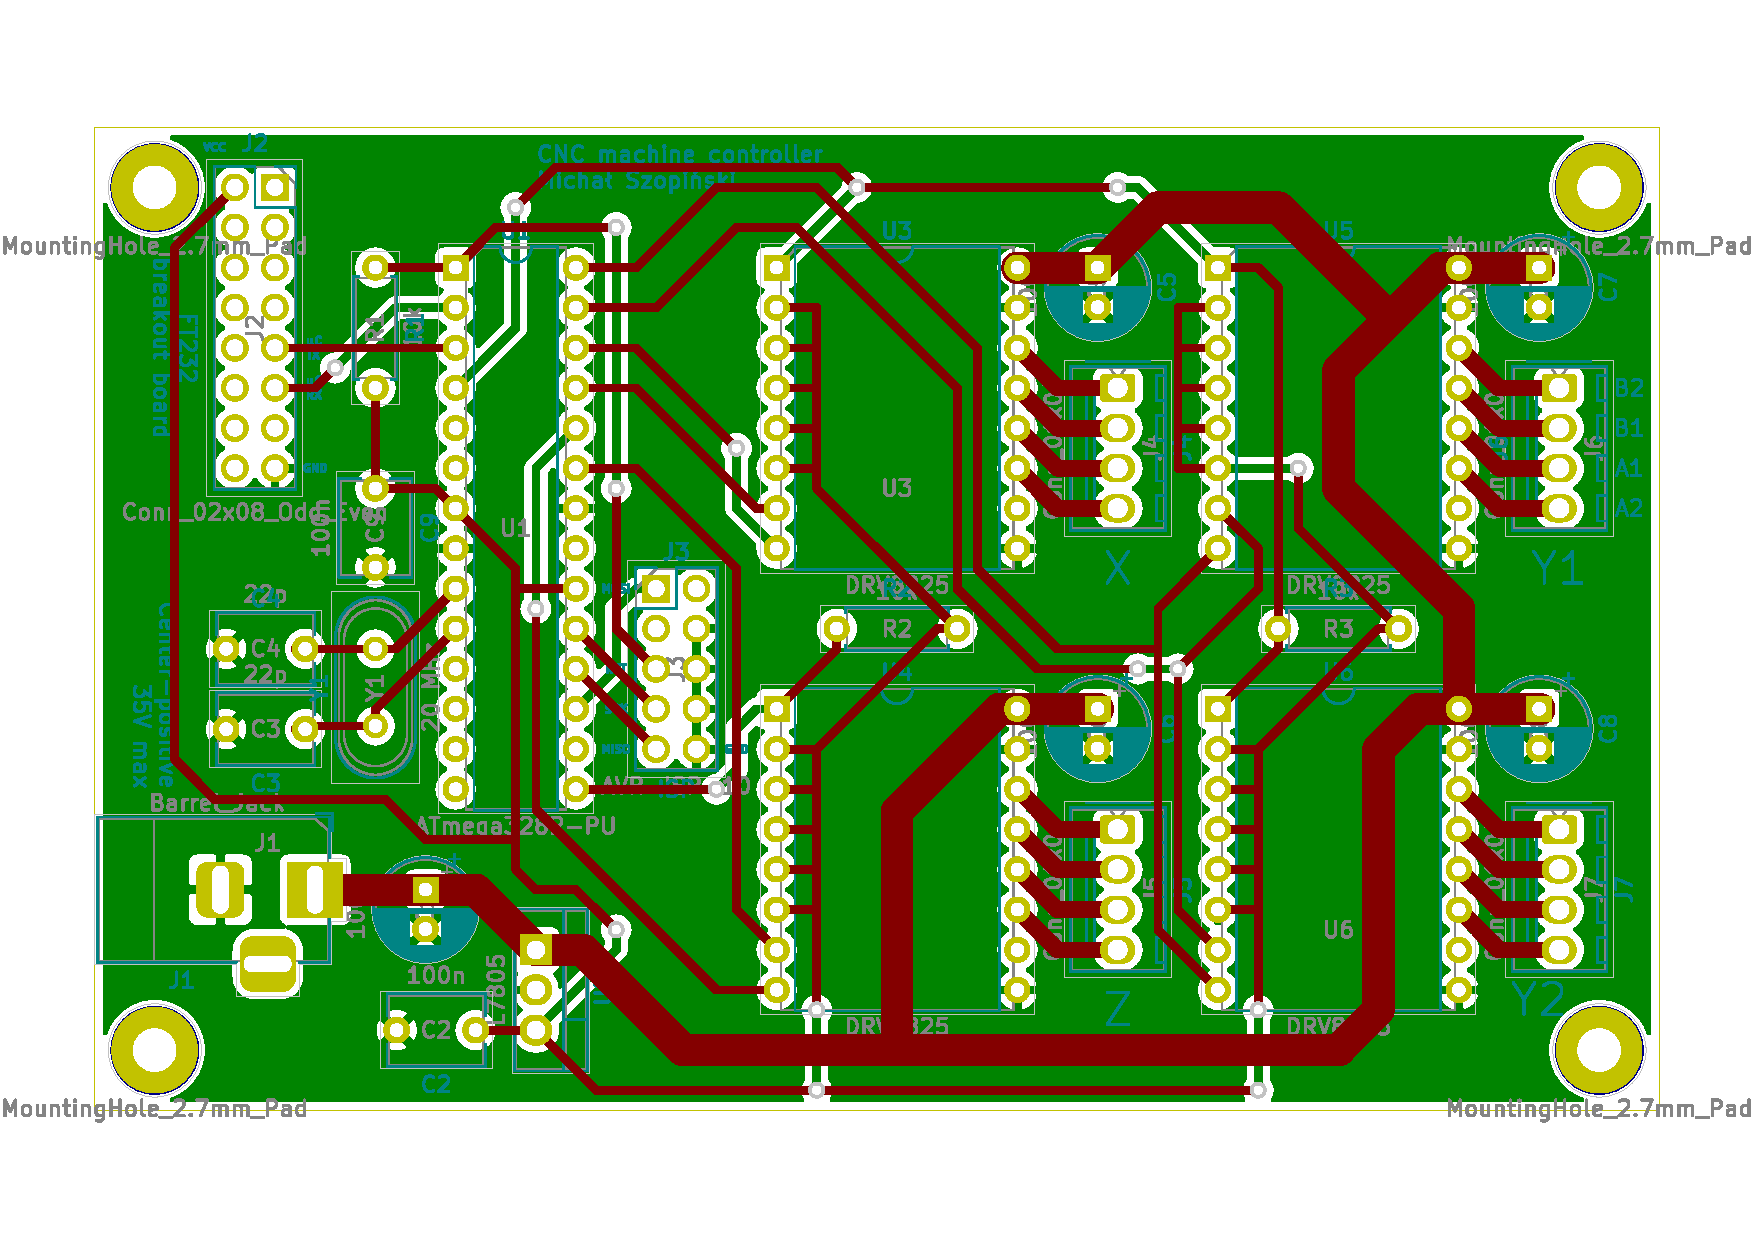
\includegraphics[width=1\linewidth]{pcb}
        \caption{Schematic of the designed PCB}
        \label{pcb}
    \end{center}
\end{figure}
\begin{figure}[ht]
    \begin{center}
        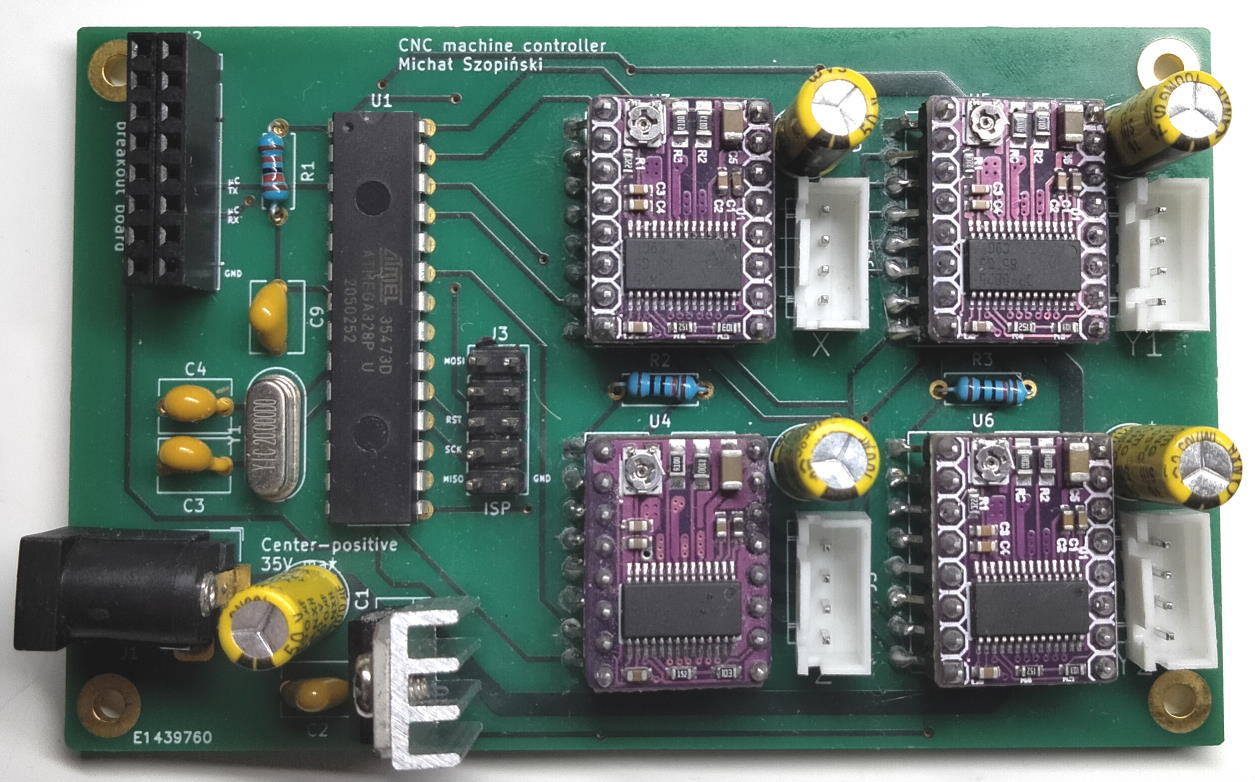
\includegraphics[width=1\linewidth]{pcb_photo}
        \caption{The designed PCB, assembled}
        \label{pcb_photo}
    \end{center}
\end{figure}
\clearpage
